
\section{Case Study: deep-sequenced short tags}\label{hoen}
\subsection{Introduction}
This section provides a detailed analysis of data from an experiment
seeking to compare deep-sequenced tag-based expression profiling to
the microarray platforms that had been previously used to conduct such
studies~\citep{THoen:2008p9}.

\subsection{Source of the data}
\citet{THoen:2008p9} address both biological and technical questions
in their study. The biological question addressed was the
identification of transcripts differentially expressed in the
hippocampus between wild-type mice and transgenic mice overexpressing
a splice variant of the $\delta$C-doublecortin-like kinase-1
(\emph{Dclk1}) gene. The splice variant, DCLK-short, makes the kinase
constitutively active and causes subtle behavioural phenotypes.

On the technical side, the researchers compare the robustness,
resolution and inter-lab portability of Solexa/Illumina's DGE tag
profiling approach and five microarray
platforms~\citep{THoen:2008p9}. The tag-based gene expression
technology in this experiment could be thought of as a hybrid between
SAGE and RNA-seq---like SAGE it uses short sequence tags ($\sim17$bp)
to identify transcripts, but it uses the deep sequencing capabilities
of Solexa/Illumina 1G Genome Analyzer to greatly increase the number
of tags that can be sequenced. For our purposes we will concentrate
solely on the DGE data generated in the experiment.

The RNA samples came from wild-type male C57/BL6j mice and transgenic
mice overexpressing DCLK-short with a C57/BL6j background. Tissue
samples were collected from four individuals in each of the two groups
by dissecting out both hippocampi from each mouse. Total RNA was
isolated and extracted from the hippocampus cells and sequence tags
were prepared using Illumina's Digital Gene Expression Tag Profiling
Kit according to the manufacturer's protocol.

Sequencing was done using Solexa/Illumina's Whole Genome
Sequencer. RNA from each biological sample was supplied to an
individual lane in one Illumina 1G flowcell. The instrument conducted
$18$ cycles of base incorporation, then image analysis and basecalling
were performed using the Illumina Pipeline. Sorting and counting the
unique tags followed, and the raw data (tag sequences and counts) are
what we will analyze here. \citet{THoen:2008p9} went on to annotate
the tags by mapping them back to the genome. In general, the mapping
of tags is an important and highly non-trivial part of a DGE
experiment, but we shall not deal with this task in this case study.

The researchers obtained $\sim2.4$ million sequence tags per sample,
with tag abundance spanning four orders of magnitude. They found the
results to be highly reproducible, even across laboratories. Using a
dedicated Bayesian model, they found $3179$ transcripts to be
differentially expressed with a FDR of $8.5$\%. This is a much higher
figure than was found for the microarrays. \citet{THoen:2008p9}
conclude that deep-sequencing offers a major advance in robustness,
comparability and richness of expression profiling data.


\subsection{Reading in the data and creating a \code{DGEList} object}
Our first task is to load the \edgeR~package, read the data into
\R~and organise the data into an object that the functions in the
package can recognise. In this case, the tag counts for the eight
individual libraries are stored in eight separate plain text files,
\code{GSM272105.txt}, \code{GSM272106.txt}, \code{GSM272318.txt},
\code{GSM272319.txt}, \code{GSM272320.txt}, \code{GSM272321.txt},
\code{GSM272322.txt} and \code{GSM272323.txt}.

In each file, the tag IDs and counts for each tag are provided in a
table. It is best to create a tab-delimited, plain-text `Targets'
file, which, under the headings `files', `group' and `description',
gives the filename, the group and a brief description for each sample.

The \code{targets} object is produced when the `Targets.txt' file is
read into the \code{R} session. This object makes a convenient
argument to the function \code{readDGE} which reads the tables of
counts into our \code{R} session, calculates the sizes of the count
libraries and produces a \code{DGEList} object for use by subsequent
functions.

\begin{Schunk}
\begin{Sinput}
> path <- getwd()
> setwd("/Users/dmccarthy/Documents/DGE/Long_SAGE_Data")
> library(edgeR)
> targets <- read.delim(file = "targets.txt", stringsAsFactors = FALSE)
> targets
\end{Sinput}
\begin{Soutput}
          files group                          description
1 GSM272105.txt  DCLK transgenic (Dclk1) mouse hippocampus
2 GSM272106.txt    WT          wild-type mouse hippocampus
3 GSM272318.txt  DCLK transgenic (Dclk1) mouse hippocampus
4 GSM272319.txt    WT          wild-type mouse hippocampus
5 GSM272320.txt  DCLK transgenic (Dclk1) mouse hippocampus
6 GSM272321.txt    WT          wild-type mouse hippocampus
7 GSM272322.txt  DCLK transgenic (Dclk1) mouse hippocampus
8 GSM272323.txt    WT          wild-type mouse hippocampus
\end{Soutput}
\begin{Sinput}
> d <- readDGE(targets, skip = 5, comment.char = "!")
> d
\end{Sinput}
\begin{Soutput}
An object of class "DGEList"
$samples
          files group                          description lib.size
1 GSM272105.txt  DCLK transgenic (Dclk1) mouse hippocampus  2685418
2 GSM272106.txt    WT          wild-type mouse hippocampus  3517977
3 GSM272318.txt  DCLK transgenic (Dclk1) mouse hippocampus  3202246
4 GSM272319.txt    WT          wild-type mouse hippocampus  3558260
5 GSM272320.txt  DCLK transgenic (Dclk1) mouse hippocampus  2460753
6 GSM272321.txt    WT          wild-type mouse hippocampus   294909
7 GSM272322.txt  DCLK transgenic (Dclk1) mouse hippocampus   651172
8 GSM272323.txt    WT          wild-type mouse hippocampus  3142280
  norm.factors
1            1
2            1
3            1
4            1
5            1
6            1
7            1
8            1

$counts
                  1 2 3 4 5 6 7 8
CATCGCCAGCGGGCACC 1 0 0 0 0 0 0 0
AAGGTCGACTCTGAAGT 1 1 0 0 0 0 0 0
CCTTCCTGGCTCTATGG 1 0 0 0 0 0 0 0
TCTGCTGAGCGTCTGTT 1 0 0 0 0 0 0 0
CCCCAGAGCGAATCAGG 1 1 2 1 1 0 2 1
844311 more rows ...
\end{Soutput}
\begin{Sinput}
> colnames(d) <- c("DCLK1", "WT1", "DCLK2", "WT2", "DCLK3", "WT3", 
+     "DCLK4", "WT4")
> setwd(path)
\end{Sinput}
\end{Schunk}

This \code{DGEList} is now ready to be passed to the functions that do
the calculations to determine differential expression levels for the
genes. Note that when we `see' the \code{DGEList} object \code{d}, the
counts for just the first five genes in the table are shown, as well
as the \code{samples} element, which is a data frame constructed from
the `Targets.txt' file and provides the filenames, groups,
descriptions and library sizes for the samples.

However, for this dataset, there were over 800 000 unique tags
sequenced, most of which have a very small number of counts in total
across all libraries. Since it is not possible to achieve statistical
significance with fewer than six counts in total for a tag, we filter
out tags which have fewer than one count per million in five or more
libraries.  This reduces our chances of finding spurious DE (that is,
DE driven by large counts in only a handful of libraries) and also
helps to speed up the calculations we need to perform. The subsetting
capability of \code{DGEList} objects makes such filtering very easy to
carry out.

\begin{Schunk}
\begin{Sinput}
> d <- d[rowSums(1e+06 * d$counts/expandAsMatrix(d$samples$lib.size, 
+     dim(d)) > 1) >= 3, ]
> dim(d)
\end{Sinput}
\begin{Soutput}
[1] 53842     8
\end{Soutput}
\end{Schunk}

Now the dataset is ready to be analysed for differential expression,
with just over $53000$ tags remaining with sufficient expression for
meaningful DE analysis.


\subsection{Producing an MDS plot}
Before proceeding with the computations for differential expression,
it is possible to produce a plot showing the sample relations based on
multidimensional scaling. The function \code{plotMDS.dge} produces an
MDS plot for the samples when provided with the \code{DGEList} object
and other usual graphical parameters as arguments, as shown below.

\begin{Schunk}
\begin{Sinput}
> pdf(file = "edgeR_case_study_longSAGE_MDSplot.pdf", height = 6, 
+     width = 6)
> plotMDS.dge(d, main = "MDS Plot for 't Hoen Data", xlim = c(-2, 
+     1))
\end{Sinput}
\begin{Soutput}
Using grid search to estimate tagwise dispersion. 
\end{Soutput}
\begin{Sinput}
> dev.off()
\end{Sinput}
\begin{Soutput}
null device 
          1 
\end{Soutput}
\end{Schunk}

This function is a variation on the usual multdimensional scaling (or
principle coordinate) plot, in that a distance measure particularly
appropriate for the digital gene expression (DGE) context is used. The
distance between each pair of samples (columns) is the square root of
the common dispersion for the top $n$ (default is $n = 500$) genes
which best distinguish that pair of samples. These top $n$ genes are
selected according to the tagwise dispersion of all the samples. The
resulting plot for the `t Hoen data is shown
in~\ref{fig:tHoen_MDS}. 

\begin{figure}[ht]
\begin{center}
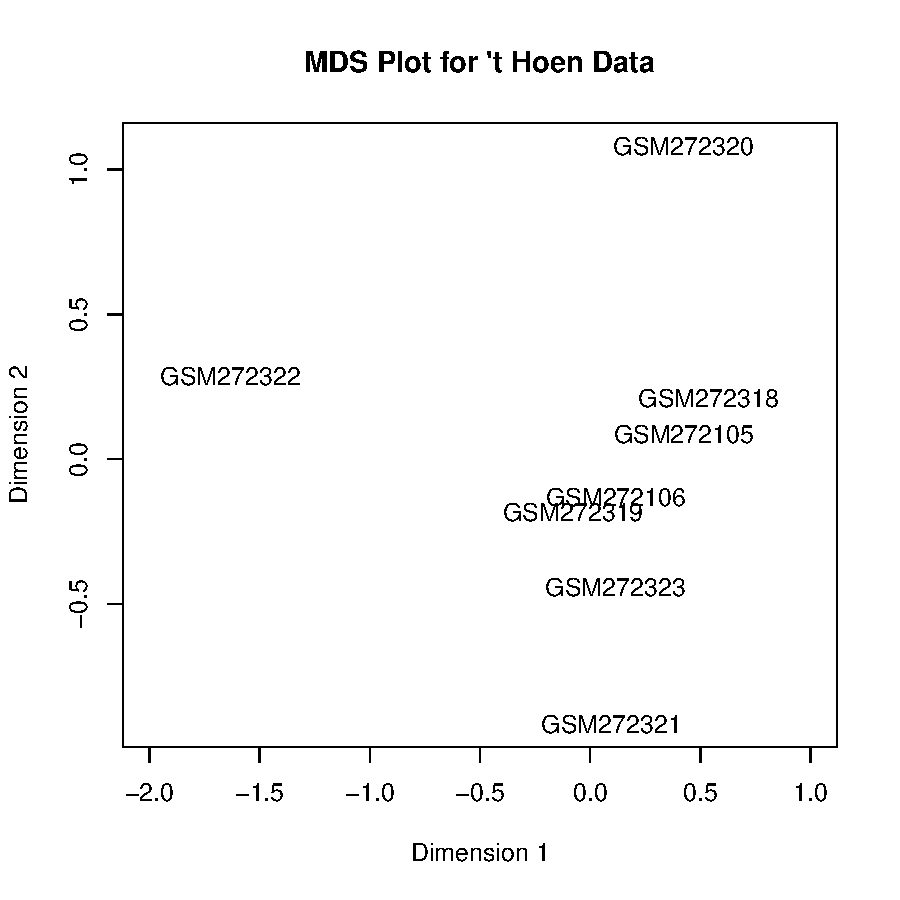
\includegraphics[height=0.45\textheight]{edgeR_case_study_longSAGE_MDSplot.pdf}
\caption{Multidimensional scaling (MDS) plot for the `t Hoen data,
  showing the relations between the samples in two
  dimensions. Dimension 1 separates the DCLK and WT samples quite nicely.}
\label{fig:tHoen_MDS}
\end{center}
\end{figure}



\subsection{Analysis using common dispersion}
\subsubsection{Estimating the common dispersion}
As discussed for the SAGE data, the first major step in the analysis
of DGE data using the NB model is to estimate the dispersion parameter
for each tag. Like in the earlier case study, we begin by estimating
the common dispersion using the function \code{estimateCommonDisp}.

\begin{Schunk}
\begin{Sinput}
> system.time(d <- estimateCommonDisp(d))
\end{Sinput}
\begin{Soutput}
   user  system elapsed 
 24.835  16.578  42.269 
\end{Soutput}
\begin{Sinput}
> names(d)
\end{Sinput}
\begin{Soutput}
[1] "samples"           "common.dispersion" "counts"           
[4] "pseudo.alt"        "genes"             "all.zeros"        
[7] "conc"              "common.lib.size"  
\end{Soutput}
\end{Schunk}

We see in the output below that the total counts in each library of
the pseudocounts agrees well with the common library size, as desired.

\begin{Schunk}
\begin{Sinput}
> d$samples$lib.size
\end{Sinput}
\begin{Soutput}
[1] 2685418 3517977 3202246 3558260 2460753  294909  651172 3142280
\end{Soutput}
\begin{Sinput}
> d$common.lib.size
\end{Sinput}
\begin{Soutput}
[1] 1885653
\end{Soutput}
\begin{Sinput}
> colSums(d$pseudo.alt)
\end{Sinput}
\begin{Soutput}
  DCLK1     WT1   DCLK2     WT2   DCLK3     WT3   DCLK4     WT4 
1730559 1730394 1722869 1717904 1724596 1736061 1758558 1730391 
\end{Soutput}
\end{Schunk}

Here the coefficient of variation of biological variation (square root
of the common dispersion) is found to be $0.40$. We also note that a
common dispersion estimate of $0.16$ means that there is a lot more
variability in the data that can be accounted for by the Poisson
model---if a tag has just $200$ counts in total (average of 25 counts
per sample), then the estimate of the tag's variance under the NB
model is over $10$ times greater than it would be under the Poisson
model.

\begin{Schunk}
\begin{Sinput}
> d$common.dispersion
\end{Sinput}
\begin{Soutput}
[1] 0.161519
\end{Soutput}
\begin{Sinput}
> sqrt(d$common.dispersion)
\end{Sinput}
\begin{Soutput}
[1] 0.4018942
\end{Soutput}
\end{Schunk}

\subsubsection{Testing}
Once we have an estimate of the common dispersion, we can proceed with
testing procedures for determining differential expression. As for the
SAGE data, there are only two groups here, so the pair need not be
specified in the call to \code{exactTest}.

\begin{Schunk}
\begin{Sinput}
> system.time(de.common <- exactTest(d))
\end{Sinput}
\begin{Soutput}
Comparison of groups:  WT - DCLK 
   user  system elapsed 
 26.713   7.991  34.932 
\end{Soutput}
\end{Schunk}

The results of the NB exact test can be accessed conveniently using
the \code{topTags} function applied to the object produced by
\code{exactTest}. The table below shows the top $10$ DE genes ranked
by $p$-value.

The table in the output from \code{topTags} shows that the
\edgeR~package identifies a good deal of differential expression
between the wild-type and the DCLK-transgenic groups. The top DE tags
are given very small $p$-values, even after adjusting for multiple
testing. Furthermore, all of the top tags have a large fold change,
indicating that these tags are likely to be biologically
meaningful. As suggested in the SAGE case study, a Gene Ontology
analysis could be carried out using the list of top tags and
$p$-values provided by \code{topTags} in order to obtain more
systematic and functional information about the differentially
expressed genes.

\begin{Schunk}
\begin{Sinput}
> topTags(de.common)
\end{Sinput}
\begin{Soutput}
Comparison of groups: WT-DCLK 
                    logConc      logFC       PValue          FDR
AATTTCTTCCTCTTCCT -17.29940  11.605637 3.740474e-43 2.013946e-38
CCGTCTTCTGCTTGTCG -10.57557   5.566736 1.246162e-28 3.354793e-24
TCTGTACGCAGTCAGGC -18.46446  -9.732358 8.588672e-26 1.232375e-21
CCGTCTTCTGCTTGTAA -14.44493   5.425811 9.155493e-26 1.232375e-21
CCGTCTTCTGCTTGTCA -15.46499   5.469611 1.008337e-23 1.085818e-19
AAGACTCAGGACTCATC -32.26560  35.500911 1.338780e-22 1.201377e-18
CCGTCTTCTGCTTGTAG -15.58127   4.761123 6.560131e-20 5.045866e-16
AGTGTGACGTGACCGGG -19.05893   8.075424 2.546566e-19 1.713903e-15
AAATTCTTCCTCTTCCT -19.14120   7.922030 2.439687e-18 1.459529e-14
CATAAGTCACAGAGTCG -32.76212 -34.507864 1.573506e-15 8.472070e-12
\end{Soutput}
\end{Schunk}

The table below shows the raw counts for the tags that \edgeR~has
identified as the most differentially expressed. For these tags there
seem to be very large differences between the groups, suggesting that
the DE genes identified are truly differentially expressed, and not
false positives. We do see, however, that when a common dispersion
value is used, tags which have just one large count in one sample can
appear as highly DE. If we wish to give less significance to such tags
then we can use tagwise dispersion estimates as described below.

\begin{Schunk}
\begin{Sinput}
> detags.com <- rownames(topTags(de.common)$table)
> d$counts[detags.com, order(d$samples$group)]
\end{Sinput}
\begin{Soutput}
                  DCLK1 DCLK2 DCLK3 DCLK4  WT1 WT2  WT3  WT4
AATTTCTTCCTCTTCCT     1     0     0     0   44   1   76 3487
CCGTCTTCTGCTTGTCG   106   268   601     5 1485 420 5156  242
TCTGTACGCAGTCAGGC   160   101   440    33    0   1    0    0
CCGTCTTCTGCTTGTAA    12    21    31     1   87  28  352   14
CCGTCTTCTGCTTGTCA     2     8    19     1   42  17  183   17
AAGACTCAGGACTCATC     0     0     0     0    6   2    4  461
CCGTCTTCTGCTTGTAG     9    11    17     0   61  20  133    9
AGTGTGACGTGACCGGG     0     0     1     0  249   2    5   85
AAATTCTTCCTCTTCCT     1     0     0     0    6   0    2  288
CATAAGTCACAGAGTCG    67    77    58     7    0   0    0    0
\end{Soutput}
\end{Schunk}

If we order the tags by fold change instead of $p$-value, as in the
table below, we see that the genes with the largest fold changes have
very small concentrations, and in general the $p$-values are not as
small as when ranked by $p$-value (not surprisingly). This ranking is
dominated by genes that have zero total counts in one group and is
less informative than ranking by $p$-value.

\begin{Schunk}
\begin{Sinput}
> topTags(de.common, sort.by = "logFC")
\end{Sinput}
\begin{Soutput}
Comparison of groups: WT-DCLK 
                    logConc     logFC       PValue          FDR
AAGACTCAGGACTCATC -32.26560  35.50091 1.338780e-22 1.201377e-18
CATAAGTCACAGAGTCG -32.76212 -34.50786 1.573506e-15 8.472070e-12
ACTCTGTGTATTACTCC -32.88687  34.25837 9.030305e-15 4.420088e-11
AAAAGAAATCACAGTTG -32.96478 -34.10256 3.081569e-13 9.759871e-10
GAAATTCTCCATTGATT -33.13284  33.76643 2.687253e-13 9.042941e-10
TAAAGTTTTTTTTTTCT -33.27022  33.49168 9.120874e-12 1.888793e-08
CGCTGTCTGAGAATGAG -33.30217  33.42777 1.728567e-11 3.323911e-08
CAAACTAGAAGACAGAA -33.33060 -33.37091 2.741087e-10 3.513944e-07
CTGGCCAGCCTTTGTTG -33.37249  33.28713 5.210910e-11 9.050510e-08
AGTTTGTGGACGTTGTG -33.42512  33.18187 2.664817e-10 3.513944e-07
\end{Soutput}
\end{Schunk}

Using their dedicated Bayesian model, \citet{THoen:2008p9} found
$3179$ transcripts to be differentially expressed with a FDR of
$8.5$\%. We can compare \citet{THoen:2008p9}'s results with the
results from \edgeR~by applying the \code{topTags} function to help
look at the tags that have a FDR of less than $0.085$ after adjusting
for multiple testing using \citet{Benjamini95}'s method for
controlling the FDR.

We see in the output below that $2270$ tags ($4.2$\% of the total
number analysed) are significantly differentially expressed according
to \edgeR~using the common dispersion estimate. Of those tags, $783$
($34$\% of the DE tags) are up-regulated in the wild-type compared
with the transgenic samples and $1487$ ($66$\%) are down-regulated in
the wild-type compared with transgenic mice.

\begin{Schunk}
\begin{Sinput}
> summary(decideTestsDGE(de.common, p.value = 0.085))
\end{Sinput}
\begin{Soutput}
   [,1] 
-1  1487
0  51572
1    783
\end{Soutput}
\end{Schunk}

\subsubsection{Visualising DGE results}
The code for producing the default fold-change plot, with the top
$500$ most DE tags highlighted in red, is shown below, and the result
of this code is shown in Figure~\ref{fig:longSAGE_FC1}. In
Figure~\ref{fig:longSAGE_FC1}, we see that the $500$ tags identified
as most differentially expressed have large fold changes---almost all
of the $500$ tags in red fall outside the blue lines at $\log
\textrm{FC} = -2$ and $\log \textrm{FC} = 2$. This means that most of
these tags show at least a 4-fold change in expression level between
the samples. This plot suggests strongly that the tags identified by
\edgeR~as differentially expressed are truly differentially expressed,
and, given the large changes in expression level, are likely to be
biologically meaningful.

\begin{Schunk}
\begin{Sinput}
> detags500.com <- rownames(topTags(de.common, n = 500)$table)
> png(file = "edgeR_case_study_longSAGE-015.png", height = 600, 
+     width = 600)
> plotSmear(de.common, de.tags = detags500.com, main = "FC plot using common dispersion", 
+     cex = 0.6)
> abline(h = c(-2, 2), col = "dodgerblue", lwd = 2)
> dev.off()
\end{Sinput}
\begin{Soutput}
null device 
          1 
\end{Soutput}
\end{Schunk}

\begin{figure}[ht]
\begin{center}
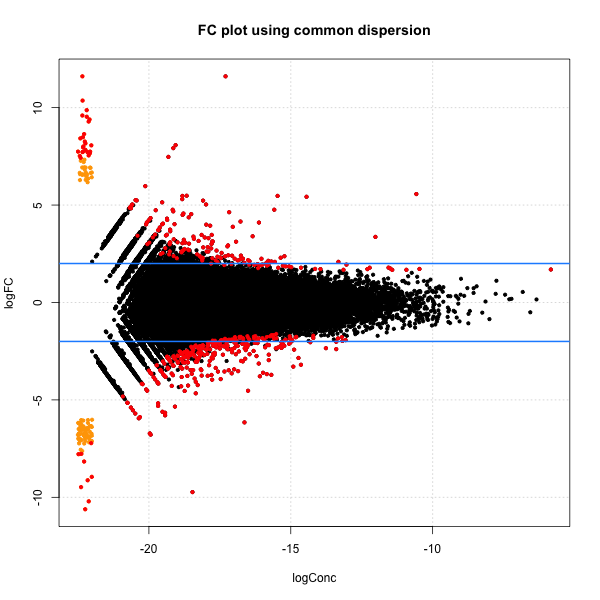
\includegraphics[height=0.45\textheight]{edgeR_case_study_longSAGE-015.png}
\caption{Plot of the log-fold change against the log-concentration for each tag. The $500$ most differentially expressed tags as identified by \edgeR~using the common dispersion are outlined in red.}
\label{fig:longSAGE_FC1}
\end{center}
\end{figure}


\subsection{Analysis using moderated tagwise dispersions}
\subsubsection{Moderating the tagwise dispersion}
An extension to simply using the common dispersion for each tag is to
estimate the dispersion separately for each tag, while `squeezing'
these estimates towards the common dispersion estimate in order to
improve inference by sharing information between tags. This type of
analysis can also be carried out in few steps using the
\edgeR~package.

To run the moderated analysis, we need to determine how much
moderation is necessary. As discussed in the SAGE case study, above,
we currently recommend choosing a
value for \code{prior.n} \emph{a priori} that will provide an
appropriate balance between the common and tagwise dispersion
values. This moderation can improve the analysis by giving higher
levels of significance to tags which have more consistent counts
within groups (and therefore lower within-group variance) and reducing
the significance of tags which have one extremely large count in one
library, which can otherwise dominate the statistical assessment of
differential expression. 


In an experiment such as that we consider here, in which we have eight
samples and thus six degrees of freedom for estimating the dispersion
parameter, setting the \code{prior.n} to be ten should be
appropriate. This means that the common likelihood receives the weight
of ten individual tags, so there will be a reasonable degree of
`squeezing' towards the common dispersion estimate, but there is still
enough scope to estimate an individual dispersion for each tag.

The function \code{estimateTagwiseDisp} produces a DGEList object that
contains all of the elements present in the object produced by
\code{estimateCommonDisp}, as well as the value for \code{prior.n}
used (\code{d\$prior.n}) and the tagwise dispersion estimates
(\code{d\$tagwise.dispersion}), as we see below. By setting the
argument \code{trend=TRUE} in the call to
\code{estimateTagwiseDisp} below we can also add an
expression-dependent trend to the ``common'' dispersion values to
which we squeeze the tagwise dispersions, by including only tags with
a similar expression level in the common likelihood for the estimation
of each tagwise dispersion.

\begin{Schunk}
\begin{Sinput}
> system.time(d <- estimateTagwiseDisp(d, prior.n = 8, prop.used = 0.3, 
+     trend = TRUE, grid.length = 500))
\end{Sinput}
\begin{Soutput}
Using grid search to estimate tagwise dispersion. 
   user  system elapsed 
 75.149  18.466  95.544 
\end{Soutput}
\begin{Sinput}
> names(d)
\end{Sinput}
\begin{Soutput}
 [1] "samples"            "common.dispersion"  "prior.n"           
 [4] "tagwise.dispersion" "counts"             "pseudo.alt"        
 [7] "genes"              "all.zeros"          "conc"              
[10] "common.lib.size"   
\end{Soutput}
\begin{Sinput}
> d$prior.n
\end{Sinput}
\begin{Soutput}
[1] 8
\end{Soutput}
\begin{Sinput}
> head(d$tagwise.dispersion)
\end{Sinput}
\begin{Soutput}
[1] 0.2062726 0.2180268 0.1947431 0.2642225 0.1248594 0.2033694
\end{Soutput}
\end{Schunk}

It is interesting to consider the distribution of the tagwise
dispersion estimates. As we can see from the output below, the tagwise
dispersion estimates range from a minimum of $0.09$ to a maximum of
$0.68$, and the common dispersion estimate lies in between the median
and mean values for the tagwise dispersion
estimates. Figure~\ref{fig:longSAGE-tgw-disp-vs-logconc} shows the
relationship between the estimated tagwise dispersions and tag
abundance (log-concentration) for this dataset.
 

\begin{Schunk}
\begin{Sinput}
> summary(d$tagwise.dispersion)
\end{Sinput}
\begin{Soutput}
   Min. 1st Qu.  Median    Mean 3rd Qu.    Max. 
 0.1001  0.1587  0.2092  0.2046  0.2392  0.7212 
\end{Soutput}
\begin{Sinput}
> d$common.dispersion
\end{Sinput}
\begin{Soutput}
[1] 0.161519
\end{Soutput}
\begin{Sinput}
> png(file = "edgeR_case_study_tHoen_tgw_disp_vs_logconc.png", 
+     height = 600, width = 600)
> plot(log(d$conc$conc.common), d$tagwise.dispersion, panel.first = grid(), 
+     ylab = "tagwise dispersion", xlab = "logConc")
> abline(h = d$common.dispersion, col = "dodgerblue", lwd = 3)
> dev.off()
\end{Sinput}
\begin{Soutput}
null device 
          1 
\end{Soutput}
\end{Schunk}

\begin{figure}[ht]
\begin{center}
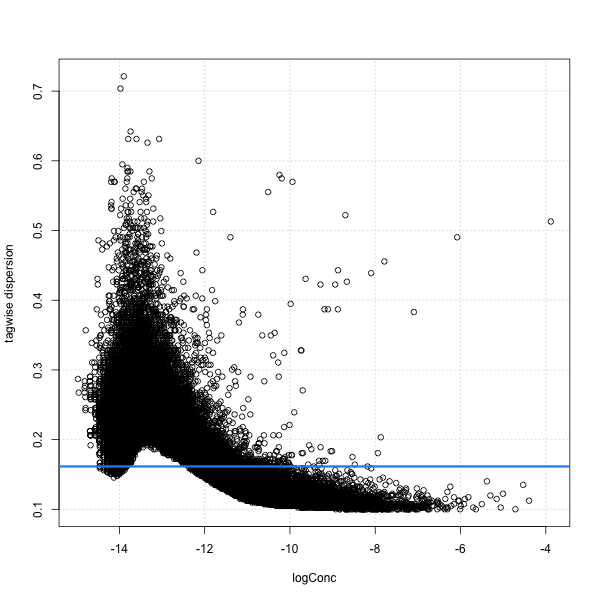
\includegraphics[height=0.45\textheight]{edgeR_case_study_tHoen_tgw_disp_vs_logconc.png}
\caption{Plot of the tagwise dispersions against tag abundance (log-concentration).}
\label{fig:longSAGE-tgw-disp-vs-logconc}
\end{center}
\end{figure}


\subsubsection{Testing}
Once we have an estimate of the common dispersion and/or estimates of
the tagwise dispersions, we can proceed with testing procedures for
determining differential expression using \code{exactTest}. Here we
carry out the testing using the tagwise dispersion estimates
calculated using a \code{prior.n} value of ten.

By default, \code{exactTest} uses the common dispersion, but by adding
the argument \code{common.disp=FALSE}, tagwise dispersion estimates
will be used instead.

\begin{Schunk}
\begin{Sinput}
> de.tagwise <- exactTest(d, common.disp = FALSE)
\end{Sinput}
\begin{Soutput}
Comparison of groups:  WT - DCLK 
\end{Soutput}
\end{Schunk}

Just as we saw earlier, the object produced by \code{exactTest}
contains two elements. The first is a data frame (\code{table}) that
contains the elements \code{logConc}, \code{logFC} and \code{p.value}
and the second is a vector (\code{comparison}) that lists the names of
the groups being compared.

The output below shows that when using tagwise dispersions, the
\edgeR~package still identifies a lot of differential expression
between the wild-type group and the DCLK-transgenic group. The top DE
tags are given very small $p$-values, even after adjusting for
multiple testing. However, We see immediately that the $p$-values for
the top tags are many orders of magnitude greater than those for the
top tags identified using the common dispersion.

As with the analysis using the common dispersion, all of the top tags
have a large fold change, indicating that these changes in expression
are likely to be biologically meaningful, although interestingly we
see more tags ($7$ out of $10$) that are down-regulated in the
wild-type group compared with the DCLK group, which contrasts with
using the common dispersion. We note that the ranking of the tags is
different, too, and only three of the top ten tags according to using
the common dispersion are found to be among the top ten tags using
tagwise dispersions.

\begin{Schunk}
\begin{Sinput}
> topTags(de.tagwise)
\end{Sinput}
\begin{Soutput}
Comparison of groups: WT-DCLK 
                    logConc      logFC       PValue          FDR
TCTGTACGCAGTCAGGC -18.46414  -9.732521 9.086167e-27 4.892174e-22
AATTTCTTCCTCTTCCT -17.30162  11.604816 3.581428e-20 9.641562e-16
CATAAGTCACAGAGTCG -32.75991 -34.512294 5.033695e-16 9.034140e-12
GCTAATAAATGGCAGAT -14.90218  -3.275617 1.446410e-15 1.946941e-11
ATACTGACATTTCGTAT -16.76738   4.163641 2.654657e-15 2.858640e-11
TCTGTATGTTCTCGTAT -16.12021   4.106937 3.934108e-15 3.530338e-11
AGTGTGACGTGACCGGG -19.06518   8.058516 6.122453e-15 4.709216e-11
CCTATTTTTCTCTCGTA -14.63299  -3.188797 3.485921e-14 2.346112e-10
TATTTTGTTTTGTCGTA -17.03685   3.883049 1.427754e-13 8.541459e-10
AAGACTCAGGACTCATC -32.28255  35.467000 1.666800e-13 8.974385e-10
\end{Soutput}
\end{Schunk}

The tables below shows the raw counts for the genes that \edgeR~has
identified as the most differentially expressed, using the common
dispersion and tagwise dispersions. For these tags, using both
methods, there seem to be very large differences between the groups,
suggesting that the DE genes identified are truly differentially
expressed, and not false positives.

Particularly noteworthy, however, is how much more consistent the
counts \emph{within} groups are for the top tags identified using
tagwise dispersions compared with those identified using the common
dispersion. This is to be expected, as allowing tagwise dispersions
penalises highly variable tags, so those that have greater variability
within groups (especially one or two libraries with extremely high
counts) will appear far lower in the ranking using tagwise dispersions
than they would using the common dispersion. This difference in the
rankings provided by the two approaches to the dispersion parameter
could yield valuable information. 

In the table below we see one tag, ``AATTTCTTCCTCTTCCT'' which is
dominated by one very large count. We see that the dispersion estimate
(the last column in the table) is $0.43$ for this tag, much higher
than the common dispersion value of $0.16$. Accordingly, the $p$-value
for DE is larger than when using the common dispersion. Even with
larger dispersion value the tag still appears as highly DE, but we do
conclude that the tag has less evidence for DE than we did using the
common dispersion. We see a similar story for the tag
``AAGACTCAGGACTCATC''.

\begin{Schunk}
\begin{Sinput}
> detags.tgw <- rownames(topTags(de.tagwise)$table)
> detags.com <- rownames(topTags(de.common)$table)
> tgw.disp <- d$tagwise.dispersion
> names(tgw.disp) <- rownames(d)
> cbind(d$counts[detags.tgw, order(d$samples$group)], tgw.disp[detags.tgw])
\end{Sinput}
\begin{Soutput}
                  DCLK1 DCLK2 DCLK3 DCLK4 WT1 WT2 WT3  WT4          
TCTGTACGCAGTCAGGC   160   101   440    33   0   1   0    0 0.1534025
AATTTCTTCCTCTTCCT     1     0     0     0  44   1  76 3487 0.4265335
CATAAGTCACAGAGTCG    67    77    58     7   0   0   0    0 0.1402509
GCTAATAAATGGCAGAT   387   321   132    71  45  32   1   38 0.1198208
ATACTGACATTTCGTAT     5     5     8     1 113 228   4  104 0.1350738
TCTGTATGTTCTCGTAT     8    12     7     3  94 427   6  177 0.1507480
AGTGTGACGTGACCGGG     0     0     1     0 249   2   5   85 0.2453300
CCTATTTTTCTCTCGTA   225   463   472    33  55  55   1   37 0.1325028
TATTTTGTTTTGTCGTA    10     5     3     0  88 171   4   67 0.1428571
AAGACTCAGGACTCATC     0     0     0     0   6   2   4  461 0.3793103
\end{Soutput}
\begin{Sinput}
> d$counts[detags.com, order(d$samples$group)]
\end{Sinput}
\begin{Soutput}
                  DCLK1 DCLK2 DCLK3 DCLK4  WT1 WT2  WT3  WT4
AATTTCTTCCTCTTCCT     1     0     0     0   44   1   76 3487
CCGTCTTCTGCTTGTCG   106   268   601     5 1485 420 5156  242
TCTGTACGCAGTCAGGC   160   101   440    33    0   1    0    0
CCGTCTTCTGCTTGTAA    12    21    31     1   87  28  352   14
CCGTCTTCTGCTTGTCA     2     8    19     1   42  17  183   17
AAGACTCAGGACTCATC     0     0     0     0    6   2    4  461
CCGTCTTCTGCTTGTAG     9    11    17     0   61  20  133    9
AGTGTGACGTGACCGGG     0     0     1     0  249   2    5   85
AAATTCTTCCTCTTCCT     1     0     0     0    6   0    2  288
CATAAGTCACAGAGTCG    67    77    58     7    0   0    0    0
\end{Soutput}
\begin{Sinput}
> topTags(de.common)
\end{Sinput}
\begin{Soutput}
Comparison of groups: WT-DCLK 
                    logConc      logFC       PValue          FDR
AATTTCTTCCTCTTCCT -17.29940  11.605637 3.740474e-43 2.013946e-38
CCGTCTTCTGCTTGTCG -10.57557   5.566736 1.246162e-28 3.354793e-24
TCTGTACGCAGTCAGGC -18.46446  -9.732358 8.588672e-26 1.232375e-21
CCGTCTTCTGCTTGTAA -14.44493   5.425811 9.155493e-26 1.232375e-21
CCGTCTTCTGCTTGTCA -15.46499   5.469611 1.008337e-23 1.085818e-19
AAGACTCAGGACTCATC -32.26560  35.500911 1.338780e-22 1.201377e-18
CCGTCTTCTGCTTGTAG -15.58127   4.761123 6.560131e-20 5.045866e-16
AGTGTGACGTGACCGGG -19.05893   8.075424 2.546566e-19 1.713903e-15
AAATTCTTCCTCTTCCT -19.14120   7.922030 2.439687e-18 1.459529e-14
CATAAGTCACAGAGTCG -32.76212 -34.507864 1.573506e-15 8.472070e-12
\end{Soutput}
\end{Schunk}

We might also be interested in comparing the top-ranking genes as
identified by \edgeR~using the common dispersion and tagwise
dispersions. The output below shows, firstly, that there are three
tags that appear in the top ten most DE tags using both common and
tagwise dispersions. Secondly, we see that of the top $1000$ most DE
tags as identified using tagwise dispersions, $79$\% of these tags are
also in the list of the $1000$ most DE tags as identified using the
common dispersion. This shows that although we do get quite different
results depending on which method we use, there is still a great deal
of agreement as to which tags are DE.

\begin{Schunk}
\begin{Sinput}
> sum(rownames(topTags(de.tagwise)$table) %in% rownames(topTags(de.common)$table))
\end{Sinput}
\begin{Soutput}
[1] 5
\end{Soutput}
\begin{Sinput}
> sum(rownames(topTags(de.tagwise, n = 1000)$table) %in% rownames(topTags(de.common, 
+     n = 1000)$table))/1000 * 100
\end{Sinput}
\begin{Soutput}
[1] 78.5
\end{Soutput}
\end{Schunk}

Using their dedicated Bayesian model, \citet{THoen:2008p9} found
$3179$ transcripts to be differentially expressed with a FDR of
$8.5$\%. The output below shows that using \citet{Benjamini95}'s
approach for controlling the FDR at $8.5$\%, \edgeR~identifies $2270$
tags as DE using common dispersion and $1929$ tags as DE using tagwise
dispersions. This means that we determine $4.2$\% and $3.6$\% of
tags to be DE using common and tagwise dispersions, respectively. The
\code{decideTestsDGE} function provides a useful way to summarize DE
results after testing, as shown below.

\begin{Schunk}
\begin{Sinput}
> sum(p.adjust(de.common$table$p.value, method = "BH") < 0.085)
\end{Sinput}
\begin{Soutput}
[1] 2270
\end{Soutput}
\begin{Sinput}
> mean(p.adjust(de.common$table$p.value, method = "BH") < 0.085) * 
+     100
\end{Sinput}
\begin{Soutput}
[1] 4.21604
\end{Soutput}
\begin{Sinput}
> sum(p.adjust(de.tagwise$table$p.value, method = "BH") < 0.085)
\end{Sinput}
\begin{Soutput}
[1] 1929
\end{Soutput}
\begin{Sinput}
> mean(p.adjust(de.tagwise$table$p.value, method = "BH") < 0.085) * 
+     100
\end{Sinput}
\begin{Soutput}
[1] 3.582705
\end{Soutput}
\begin{Sinput}
> summary(decideTestsDGE(de.tagwise, p = 0.085))
\end{Sinput}
\begin{Soutput}
   [,1] 
-1  1235
0  51913
1    694
\end{Soutput}
\end{Schunk}

Of the $1929$ tags identified as DE using tagwise dispersions, $694$
($36$\%) are up-regulated in wild-type and $1235$ ($64$\%) are
up-regulated in the transgenic mice. The proportions of up- and
down-regulated genes identified using the two approaches to modeling
the dispersion are similar, but using the common dispersion identifies
slightly more tags down-regulated in wild-type mice as DE.


\subsubsection{Visualising DGE results}
As discussed earlier, the function \code{plotSmear} can be used to
generate a plot of the log-fold change against the log-concentration
for each tag (analogous to an MA-plot in the microarray context). We
identify the top $500$ most DE tags using both common dispersion and
tagwise dispersions so we can highlight them on the plots and compare
what we see. The code for producing the fold-change plots is shown
below, and the result of this code is shown in
Figure~\ref{fig:longSAGE_FC2}.

\begin{Schunk}
\begin{Sinput}
> detags500.com <- rownames(topTags(de.common, n = 500)$table)
> detags500.tgw <- rownames(topTags(de.tagwise, n = 500)$table)
> png(file = "edgeR_case_study_longSAGE-30.png", height = 800, 
+     width = 600)
> par(mfcol = c(2, 1))
> plotSmear(de.common, de.tags = detags500.com, main = "Using common dispersion")
> abline(h = c(-2, 2), col = "dodgerblue", lwd = 2)
> plotSmear(de.tagwise, de.tags = detags500.tgw, main = "Using tagwise dispersions")
> abline(h = c(-2, 2), col = "dodgerblue", lwd = 2)
> dev.off()
\end{Sinput}
\begin{Soutput}
null device 
          1 
\end{Soutput}
\end{Schunk}

In Figure~\ref{fig:longSAGE_FC2}, the top $500$ most differentially
expressed tags (those identified as significant by \edgeR~using the
common dispersion (top) and tagwise dispersions (bottom)) are
highlighted in red. Looking at Figure~\ref{fig:longSAGE_FC2}, we see
that, generally speaking, the pattern of differential expression looks
similar using the two different methods, and the tags identified as DE
have convincingly large fold changes.

\begin{figure}[ht]
\begin{center}
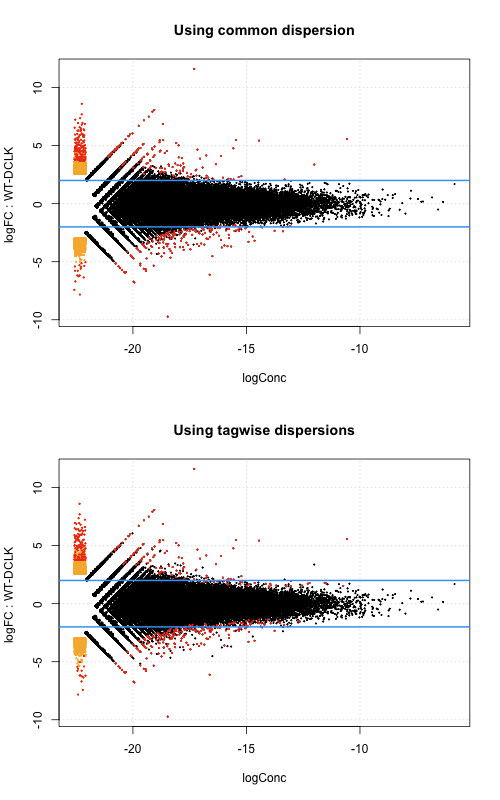
\includegraphics[height=0.8\textheight]{edgeR_case_study_longSAGE-030.png}
\caption{Plots of the log-fold change against the log-concentration for each tag, using the common dispersion (upper), and tagwise dispersions (lower). Tags with positive fold-change here are up-regulated in wild-type compared with transgenic mice. The $500$ most differentially expressed tags according to each method are highlighted in red on both plots.}
\label{fig:longSAGE_FC2}
\end{center}
\end{figure}


\subsection{Setup}
This analysis of \citet{THoen:2008p9}'s tag-based DGE data was conducted on:
\begin{Schunk}
\begin{Sinput}
> sessionInfo()
\end{Sinput}
\begin{Soutput}
R version 2.13.0 beta (2011-03-30 r55205)
Platform: i386-apple-darwin9.8.0/i386 (32-bit)

locale:
[1] C/UTF-8/C/C/C/C

attached base packages:
[1] stats     graphics  grDevices utils     datasets  methods   base     

other attached packages:
[1] edgeR_2.1.16

loaded via a namespace (and not attached):
[1] limma_3.7.26
\end{Soutput}
\end{Schunk}
and took roughly 8 minutes to carry out on an Apple MacBook with a 2.8 Ghz Intel Core 2 Duo processor and 8 Gb of 1067 MHz DDR3 memory.


